%!TEX root=../main.tex
\chapter{User and System Testing}
This chapter will explain the testing of usability of the developed system. Section \ref{sec:cont-user-testing} starts off with a brief presentation of the small continuous user testing which were concucted as new featues were implemented during the Spring. Further, section \ref{sec:user-testing} presents the motivation, methodology and results from a large scale user test conducted April 18th, and the results are compared to results gathered and presented in the Specialization report. The chapter ends with a presentation of system unit test coverage and validity. This chapter covers the following objectives presented in section \ref{sec:ps-inter}:
\begin{itemize}
  \item Conduct a user-experiment to evaluate system usability, i.e objective \texttt{U3}.
\end{itemize}

\section{Continuous User Testing}
\label{sec:cont-user-testing}

\subsection{Admin Interface Assessment}
Some system administrators were also asked to assess the usability of the improved admin interface. The admin interface usability assessment was not a part of the user test, as the user test focused on testing the frontend interface used by normal users. We also have an restrictive amount of system administrators which has been trained in how to use the interface, which makes a test of the admin interface on a wast amount of participants unnecessary.


\subsection{Validity}
\paragraph*{Admin Interface Assessment} \hfill \\
The number of admin users are small and might not be statistically significant. However, since the number of admin users is small and will stay small for some time in the future, it is important that the few admin users we have like the new admin interface improvements. Consequently, the assessment will likely be affected with experience from and observations done in the old admin interface. To improve the credability of the results one could also include testing of the admin interface in the optimal user test described above. However, this would make the user test more extensive and harder to execute, and would require a lot of administrative work.

\section{User Experiment}
\label{sec:user-testing}

\subsection{Motivation}
A user test was performed in the Specialization project and the project report were delivered in December 2015 as mentioned in sub-section \ref{subsec:related-proj}. The \gls{cmb} system was one of three tools used by the students in mandatory assignments, where the \gls{cmb} system mainly was used for testing the system on more users then previously attempted by Follan and Støa \cite{mt:T&S}. The course assignments cover various topics and methods of producing parallel code in C++, like OpenMP, NEON, MPI and CUDA, and is about 25\% of the workload during the semester for the avarage student. The TDT4200 course staff added in total 5 programming problems to \gls{cmb} which were solvable by students, and the system received a lot of submissions during the semester. \\

During November of 2015 a total of 37 students delivered an optional questionnaire which included some questions about the \gls{cmb} system. In addition to the questionnaire, some feedback on the system was gathered during the last lecture of the course late in November. The feedback were mainly focused on usability aspects of the system, which helped the \gls{cmb} project team to discover bugs, and to setup and prioritize features to implement next. The prioritized list generated a backlog, which was used as a motivation when constructing the objectives presented in section \ref{sec:ps-inter}. \\

As this thesis potentially has improved system usability, it is interesting to conduct a user study to compare the usability of the two system versions. The new system will be considered as version two in the below discussions, while the system developed by Follan and Støa will be considered as version one. As mentioned in chapter \ref{ch:design}, usability is a broad term and this thesis has contributed mainly against improving effiency, learnability, and satisfaction of users as discussed in the mentioned chapter and implemented in chapter \ref{ch:improvements}. The above observation makes it interesting to test the following hypothesis:

\paragraph*{Hypothesis 1:} The usability, in terms of either efficiency, learnability, or user satisfaction, is higher in version two compared to system verison one. \hfill \\

Further, it is interesting to investigate if the overall usability of the system has increased in the \gls{cmb} system version two i.e:

\paragraph*{Hypothesis 2:} The overall usability of system version two is higher compared to system version one. \hfill \\

\subsection{Methodology}
The user test were conducted April 18th this Spring assesses the system improvements presented in Chapter \ref{ch:improvements} with focus on usability. The goal of this second test is to further improve the results received from Specialization project user test or user test one. The second test required an interest in programming and programming experience from the participants, but no prior knowledge of C or C++ or any parallel programming libraries were set as a requirement to participate in the test. \\

The weak requirements were set since there were generally little interest from students in participating in the test. The low interest in the test is most likely due to bad timing, as many students have several assignment deliverables before the last lectures in mid April. Further, attracting students or others to participate in a user test for a master thesis is generally hard if the test takes several hours. \textit{As the focus of this test were to test the usability of the system, it should be sufficient for participants to have general knowledge and interest in programming to assess the system usability}. \\

The user test described a set of tasks to be completed by each participant. Since we are comparing the two system versions, the test does not assess the new features implemented and is assumed covered by section \ref{sec:cont-user-testing}. Appendix \ref{apdx:usertest} presents the tasks executed by every participant during the test, along with a questionnaire each participant were to complete before finishing the user test. \\

Nearly all participants conducted the test simultanously in a lecture hall to simulate the heavy submission traffic we experienced before assignment deadlines in TDT4200. A couple of participants started the user test late or participated a couple of days after the official user test, to simulate the students in TDT4200 that experienced little or no traffic. Participants were informed that questions related to how to complete a task would not be answered during the test and that tasks should be completed individually. They were also informed that they could abort the test at any time. \\

\begin{table}
    \centering
    \begin{tabular}{ | l | p{6cm} |}
    \hline
    \textbf{Problem Name} & \textbf{Problem Description Summary} \\ \hline
    Hello World & Print out "Hello World!"". \\ \hline
    Digits & \textit{T} test cases are given as input, each test case describing the range between two numbers \textit{N} and \textit{M}. For each test case, output the number of zeroes present in all the numbers in the range [\textit{N}, \textit{M}]. \\ \hline
    Prime Number & For every number in the input, output if the number is a prime. \\ \hline
    WERTYU & For every encrypted input string, decrypt it and output the decrypted string. Hint: The input strings are encrypted with an QWERTY keyboard shifted one character to the right. \\ \hline
    Reverse String & For every input string output the reversed string. \\
    \hline
    \end{tabular}
    \caption{Available Solvable Problems During User Test}
    \label{tab:avail-prob}
\end{table}

The most time consuming task the participants had to complete were to submit code to one of the problems presented in Table \ref{tab:avail-prob}. Submitting code to problems is the core of the \gls{oj} and the process of uploading and running submissions were the most common procedure done by TDT4200 students. The procedure and aspects related to submissions was also mentioned the most times in feedback given by the TDT4200 students, and was therefore chosen as one of the main tasks to perform in this user test. Before starting the user test, the participants were also notified to comment extensively on the procure when filling out the survey. \\

The participants who were unfamiliar with C and C++ were given 5 different source files to the ``Prime Number''-problem which they were to submit to the system. The thought behind handing out source files, were to simulate that the participants made a number of tries before arriving at the correct solution. The ``Prime Number''-problem were chosen as it is of medium to easy difficulty. Participants who knew either C or C++ were also motivated to try to solve more than one problem if they arrived at a solution quickly, to extensively test the procedure of uploading and running submissions. Other tasks executed by participants included sign-up, login, viewing submissions and highscore lists, joining groups, creating and administering groups, and changing user e-mail and password. \\

The questionnaire found in Appendix \ref{apdx:usertest} contains the same questions about the \gls{cmb} system presented in the questionnaire given to the students in TDT4200. The questionnaire is, as mentioned in the Specialization project report, inspired a by typical Likert scale form devloped by IBM\footnote{See: \url{http://garyperlman.com/quest/quest.cgi}} and complemented with textual based questions. To compare the results of the two questionnaires, it is important that they cover the same aspects and all questions developed in the Specialization project is therefore reused in the questionnaire handed out in this user study. In addition, a couple of extra multiple choice questions were added to the questionnaire of this test for the sake of clarity. \\

Likert scale questions are often used in usability assessment of software systems. In this test, the number of Likert scale alternatives is set to five per question. Each row in Table \ref{tab:likert-scale} shows the possible alternatives for a given question type, as well as each alternatives' corresponding score ranged from one to five. To make it easier for participants to describe their thoughts about system features, the textual based questions are provided in the questionnaire and is further used as qualitative support when discussing the user study results. \\

\begin{table}[t!]
    \centering
    \begin{tabular}{ | c | p{1.5cm} | p{1.5cm} | p{1.5cm} | p{1.5cm} | p{1.5cm} |}
    \hline
    \multirow{2}{*}{\textbf{Question Type}} & \multicolumn{5}{ c| }{\textbf{Likert Score Range}} \\ \cline{2-6}
      & 1 & 2 & 3 & 4 & 5 \\ \cline{1-6}
    A & Very poor & Poor & Neutral & Good & Very good \\ \hline
    B & Strongly disagree & Disagree & Neither agree or disagree & Agree & Strongly agree \\ \hline
    C & Very hard & Hard & Neutral & Easy & Very easy \\ \hline
    D & Not satisfied at all & A~little bit~satisfied & Neutral & Satisfied & Very satisfied \\ \hline
    \end{tabular}
    \caption{Likert Scale Alternatives on Question Type}
    \label{tab:likert-scale}
\end{table}

The tool Gnumeric \cite{GNUMERIC} is used for statistical data analysis comparison on the multiple choice results of the two user tests. Each multiple choice answer from both tests on each of the matching questions are translated into the corresponding Likert scale value. Further, a F-test \cite{moore2007} and student T-test \cite{walpole1993} is performed on each question, to determine if a two-tailed student T-test with unequal variances is needed and to determine if the two tests have significantly different means respectively. \\

If the T-test indicates a significant difference between the two user groups further analysis is needed. If so, an Anderson-Darling test \cite{razali2011} is performed to check for normality in the compared data sets, as normality is often set as a requirement for a valid T-test. However, if the normality check fails, the non-parametric Wilcoxon-Mann-Whitney test \cite{hodges2005} is performed on each of the question groups accepted by the T-test. The test is used to support the conclusion of the T-test, as non-parametric tests often are used when . \\

The statistical analysis assumes a significance level ($\alpha$) of 5\%. Further the null hypothesis ($H_0$) for the T-test assumes equal means of the two datasets, while the alternative hypothesis ($H_1$) is set depending on if we are conducting either a one-tailed or two-tailed T-test. Equation \ref{eq:h1-t-test} shows the possible alternative hypothesis for the T-test, where $\mu_{1}$ and $\mu_{2}$ are the means for user test one and two respectively.

\begin{equation} \label{eq:h1-t-test}
   H_1 =
    \begin{cases}
        \mu_{2} > \mu_{1} & \quad \text{if one-tailed test}\\
        \mu_{2} \neq \mu_{1} & \quad \text{if two-tailed test}\\
    \end{cases}
\end{equation}

The statistical effect-size is also reported and used when discussing the results. The effect-size is meant by the statistical \textit{strength} of a result, and will be important in our discussion of the multiple choice results. The reported effect-size metrics used is Cohen's d, Hedge's g, and Pearson's r \cite{cumming2013}\footnote{Calculated using this too: \url{http://www.polyu.edu.hk/mm/effectsizefaqs/calculator/calculator.html}.}. Cohen's d is often used as effect size to measure the strength of a t-test, as well as Person's r which is a well known effect-size metric. Hedge's g is also included in the results, as it is more accurate than Cohen's d with small sample sizes. \\

Table \ref{tab:effect-size} reports the size scale for each of the used effect-size metrics. Cohen's d is also used to calculate the statistical \textit{power} of a conclusion, that is, the probability of correctly rejecting $H_0$ when $H_1$ is true. Statistical power is important when discussing threats against validity, to be sure that our conclusion is correct by some probability. Statistical power of the t-test is calculated using the Real Statistics Resource Pack in Microsoft Excel \cite{RSRP}.

\begin{table}[t!]
    \centering
    \begin{tabular}{ | c | c | c | c |}
    \hline
    \textbf{Effect size} & \textbf{Pearson's r} & \textbf{Cohen's d} & \textbf{Hedge's g} \\ \hline
    Small & 0.1 & 0.2 & 0.2 \\ \hline
    Medium & 0.3 & 0.5 & 0.5 \\ \hline
    Large & 0.5 & 0.8 & 0.8 \\ \hline
    \end{tabular}
    \caption{Effect sizes and corresponding metric values}
    \label{tab:effect-size}
\end{table}

\subsection{Results and Evaluation}

\begin{figure}
    \centering
    %\hspace*{-1.5cm}
    \begin{subfigure}[h]{0.48\textwidth}
        \centerline{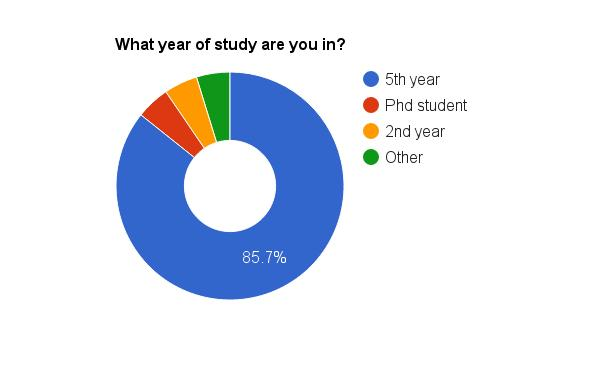
\includegraphics[width=1.5\textwidth]{results/year_of_study.jpg}}
        \caption{*}
        \label{fig:year-of-study}
    \end{subfigure}
    ~ %add desired spacing between images, e. g. ~, \quad, \qquad, \hfill etc.
      %(or a blank line to force the subfigure onto a new line)
    \hfill
    \begin{subfigure}[h]{0.48\textwidth}
        \centerline{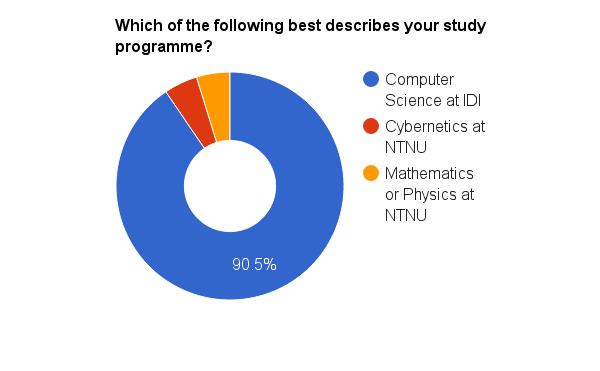
\includegraphics[width=1.5\textwidth]{results/study_programme.jpg}}
        \caption{*}
        \label{fig:study-programme}
    \end{subfigure}
    %add desired spacing between images, e. g. ~, \quad, \qquad, \hfill etc.
    %(or a blank line to force the subfigure onto a new line)

    %\hspace*{-1.5cm}
    \begin{subfigure}[h]{0.48\textwidth}
        \centerline{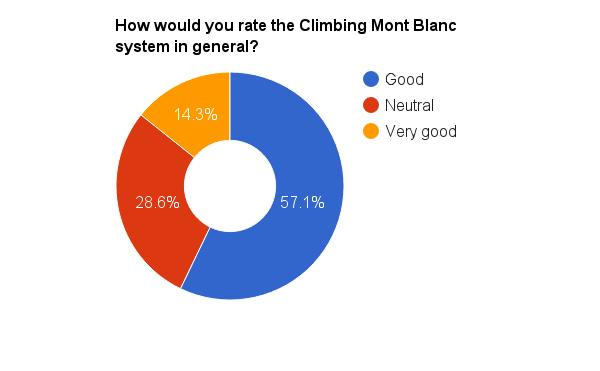
\includegraphics[width=1.5\textwidth]{results/general_cmb.jpg}}
        \caption{A1}
        \label{fig:cmb-general}
    \end{subfigure}
    \hfill
    \begin{subfigure}[h]{0.48\textwidth}
        \centerline{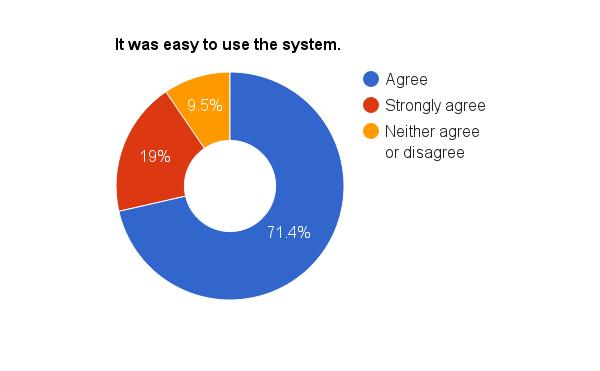
\includegraphics[width=1.5\textwidth]{results/easy_to_use.jpg}}
        \caption{B1}
        \label{fig:cmb-easy-use}
    \end{subfigure}
    \caption{Multiple Choice Results}
    \label{fig:multiplechoice}
\end{figure}


\begin{figure}
    \centering
    %\hspace*{-1.5cm}
    \begin{subfigure}[h]{0.48\textwidth}
        \centerline{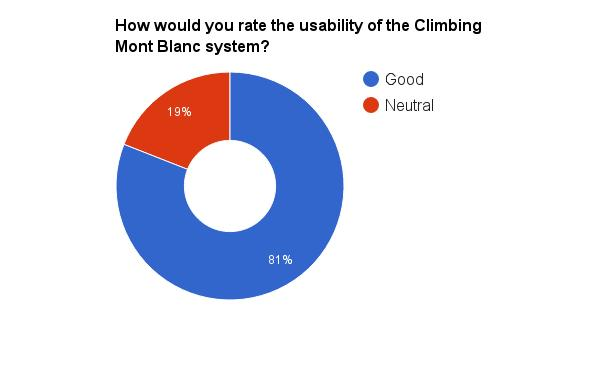
\includegraphics[width=1.5\textwidth]{results/usability_cmb.jpg}}
        \caption{A2}
        \label{fig:cmb-usability}
    \end{subfigure}
    ~ %add desired spacing between images, e. g. ~, \quad, \qquad, \hfill etc.
      %(or a blank line to force the subfigure onto a new line)
    \hfill
    \begin{subfigure}[h]{0.48\textwidth}
        \centerline{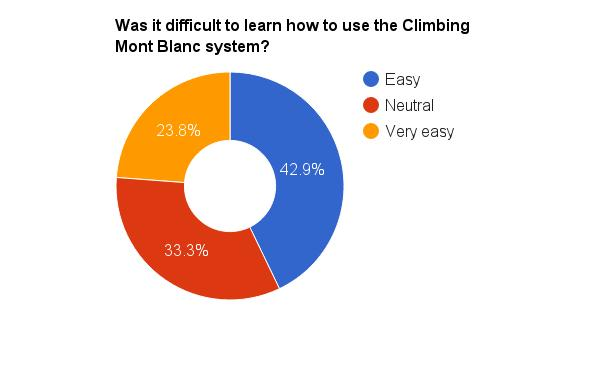
\includegraphics[width=1.5\textwidth]{results/learn_cmb.jpg}}
        \caption{C1}
        \label{fig:cmb-learn}
    \end{subfigure}

    %\hspace*{-1.5cm}
    \begin{subfigure}[h]{0.48\textwidth}
        \centerline{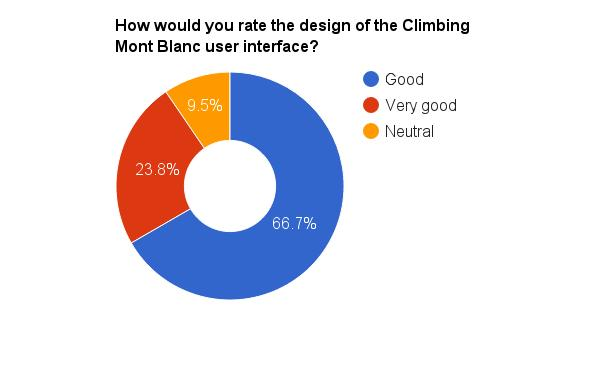
\includegraphics[width=1.5\textwidth]{results/design_cmb.jpg}}
        \caption{A3}
        \label{fig:cmb-design}
    \end{subfigure}
    ~ %add desired spacing between images, e. g. ~, \quad, \qquad, \hfill etc.
      %(or a blank line to force the subfigure onto a new line)
    \hfill
    \begin{subfigure}[h]{0.48\textwidth}
        \centerline{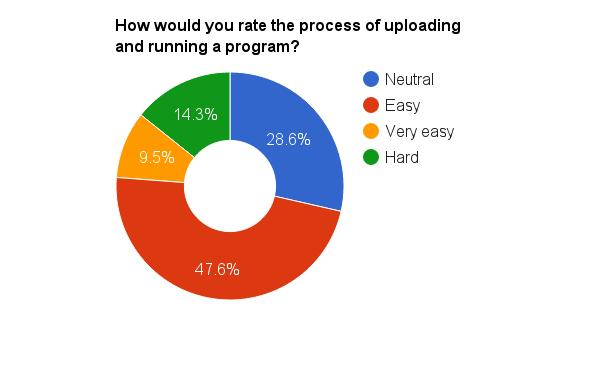
\includegraphics[width=1.5\textwidth]{results/submission_cmb.jpg}}
        \caption{C2}
        \label{fig:cmb-submission}
    \end{subfigure}
    \caption{Multiple Choice Results (continuation of Figure \ref{fig:multiplechoice})}
    \label{fig:multiplechoice1}
\end{figure}

\begin{figure}
    \centering
    %\hspace*{-1.5cm}
    \begin{subfigure}[h]{0.45\textwidth}
        \centerline{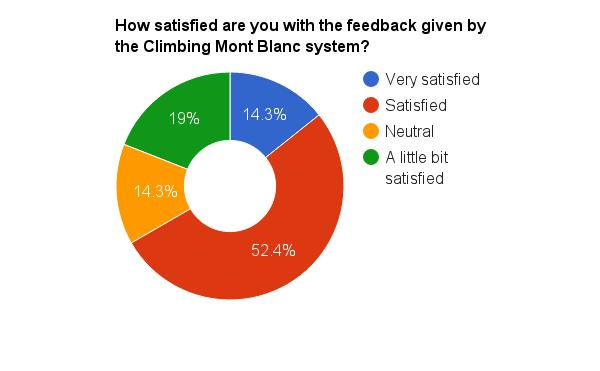
\includegraphics[width=1.5\textwidth]{results/feedback_cmb.jpg}}
        \caption{D1}
        \label{fig:cmb-feedback}
    \end{subfigure}
    \hfill
    \begin{subfigure}[h]{0.45\textwidth}
        \centerline{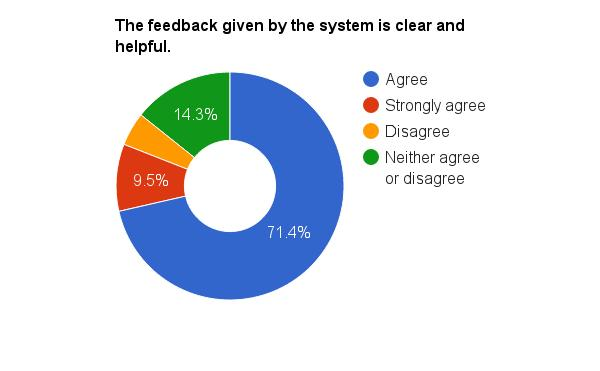
\includegraphics[width=1.5\textwidth]{results/clear_feedback_cmb.jpg}}
        \caption{B2}
        \label{fig:cmb-feedback-clear}
    \end{subfigure}

    %\hspace*{-1.5cm}
    \begin{subfigure}[h]{0.45\textwidth}
        \centerline{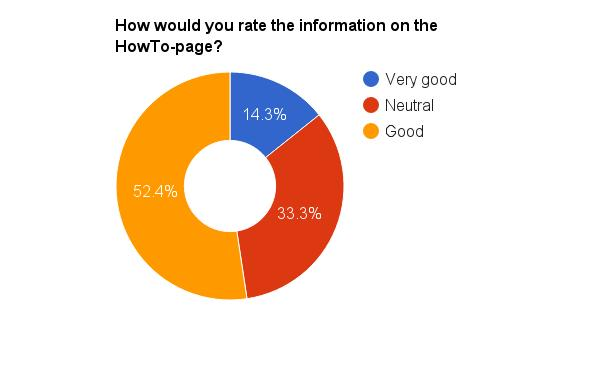
\includegraphics[width=1.5\textwidth]{results/howto_cmb.jpg}}
        \caption{A4}
        \label{fig:cmb-howto}
    \end{subfigure}
    \caption{Multiple Choice Results (continuation of Figure \ref{fig:multiplechoice1})}
    \label{fig:multiplechoice2}
\end{figure}

There were in total 21 participants in the second user test. The Figures \ref{fig:multiplechoice}, \ref{fig:multiplechoice1}, \ref{fig:multiplechoice2} shows the results of the multiplechoice Likert questions. Some sub figures is labeled according to the question types defined in Table \ref{tab:likert-scale}, to easy reference the question in the below discussion. As mentioned, there were a total of 37 TDT4200 students providing feedback in the optional questionnaire given during the Autmumn semester. The results from the user test conducted as part of the Specialization project is included in Appendix \ref{apdx:usertest}. \\

Table \ref{} shows the mean and variance of user test one and test two on each question. The table also include f-test and t-test data

\subsection{Threats to Validity}
There are multiple factors in the experimental setup and execution of this test that may threaten the internal validity of the results. First, the participants in the user test does not necessarily have the same background and interests as the students in the course TDT4200. This may have an effect on how the participants percieve the system, and it may be different from the perception made by students students in TDT4200. Most of the TDT4200 students are interested in low-level and parallel programming, and may have little interest in design or frontend functionality as long as the system is in some way usable. A possible side effect might be that the two groups perceive the system usability differently. \\

Second, the participants of this test used the system for a short period of time. The students in TDT4200 used the system in a total of 5 exercises throughout the Autumn semester, and have tried using the system multiple times. The participants in this test may not have been able to test the system thoroughly like the students in TDT4200 had a chance to do. Third, the number of participants in this test may not be as statistically significant as in the user test conducted during the Autumn. Conclusions drawn from unequal quantities of participants in the two tests may be less correct than two tests having equal amount of participants, and the reader should keep this in mind during evalution. Fourth, since it was hard to get participants to the test, many of the participants are friends of or familiar to the \gls{cmb} team. This might further affect the results in either a positive or negative way. \\


\section{System Unit Tests}

\subsection{Coverage}

\subsection{Validity}
